% Created 2025-04-04 Fri 11:54
% Intended LaTeX compiler: pdflatex
\documentclass[smaller]{article}
\usepackage[utf8]{inputenc}
\usepackage[T1]{fontenc}
\usepackage{graphicx}
\usepackage{longtable}
\usepackage{wrapfig}
\usepackage{rotating}
\usepackage[normalem]{ulem}
\usepackage{amsmath}
\usepackage{amssymb}
\usepackage{capt-of}
\usepackage{hyperref}
\usepackage{color}
\usepackage{listings}
%\useoutertheme{infolines}
\usepackage{tikz}
\usepackage{tikzsymbols}
\usepackage{amsmath}
\usepackage{amssymb}
\usepackage{mathrsfs}
\usepackage{isomath}
\usepackage{algorithmic}
\usepackage{fontawesome}
\usepackage{svg}
\newcommand \E {\mathop{\mbox{\ensuremath{\mathbb{E}}}}\nolimits}
\newcommand \Var {\mathop{\mbox{\ensuremath{\mathbb{V}}}}\nolimits}
\newcommand \Bias {\mathop{\mbox{\ensuremath{\mathbb{B}}}}\nolimits}
\newcommand\ind[1]{\mathop{\mbox{\ensuremath{\mathbb{I}}}}\left\{#1\right\}}
\newcommand{\indep}{\mathrel{\text{\scalebox{1.07}{$\perp\mkern-10mu\perp$}}}}
\renewcommand \Pr {\mathop{\mbox{\ensuremath{\mathbb{P}}}}\nolimits}
\DeclareMathOperator*{\argmax}{arg\,max}
\DeclareMathOperator*{\argmin}{arg\,min}
\DeclareMathOperator*{\sgn}{sgn}
\newcommand \defn {\mathrel{\triangleq}}
\newcommand \loss {L}
\newcommand \cost {\ell}
\newcommand \util {U}
\newcommand \trans {\tau}
\newcommand \rewrad {r}
\newcommand \Reals {\mathbb{R}}
\newcommand \Naturals {\mathbb{N}}
\newcommand \Param {\Theta}
\newcommand \param {\theta}
\newcommand \pol {\pi}
\newcommand \Pols {\Pi}
\newcommand \vparam {\vectorsym{\beta}}
\newcommand \mparam {\matrixsym{B}}
\newcommand \CX {\mathcal{X}}
\newcommand \CA {\mathcal{A}}
\newcommand \CY {\mathcal{Y}}
\newcommand \bW {\matrixsym{W}}
\newcommand \bw {\vectorsym{w}}
\newcommand \wi {\vectorsym{w}_i}
\newcommand \wij {w_{i,j}}
\newcommand \bA {\matrixsym{A}}
\newcommand \ai {\vectorsym{a}_i}
\newcommand \aij {a_{i,j}}
\newcommand \by {\vectorsym{y}}
\newcommand \hby {\vectorsym{\hat{y}}}
\newcommand \hy {\hat{y}}
\newcommand \bz {\vectorsym{z}}
\newcommand \bx {\vectorsym{x}}
\newcommand \bX {\matrixsym{X}}
\newcommand \dbel {\beta}
\newcommand \bel {\beta}
\newcommand \Bel {\mathcal{B}}
\newcommand \Ber {\textrm{Bernoulli}}
\newcommand \Unif {\textrm{Unif}}
\newcommand \Mult {\textrm{Mult}}
\newcommand \Beta {\textrm{Beta}}
\newcommand \Dir {\textrm{Dir}}
\newcommand \Normal {\textrm{Normal}}
\newcommand \Simplex {\mathbb{\Delta}}
\newcommand \outcome {\omega}
\newcommand \Outcomes {\Omega}



\newcommand \pn {\param^{(n)}}
\newcommand \pnn {\param^{(n+1)}}
\newcommand \pnp {\param^{(n-1)}}
\newcommand \parent {\texttt{par}}
\newcommand \child {\texttt{chi}}
\newcommand \anc {\texttt{anc}}


\usetikzlibrary{shapes.geometric}
\usetikzlibrary{arrows.meta, positioning, quotes}

\tikzstyle{utility}=[diamond,draw=black,draw=blue!50,fill=blue!10,inner sep=0mm, minimum size=8mm]
\tikzstyle{select}=[rectangle,draw=black,draw=blue!50,fill=blue!10,inner sep=0mm, minimum size=6mm]
\tikzstyle{hidden}=[dashed,draw=black,fill=red!10]
\tikzstyle{RV}=[circle,draw=black,draw=blue!50,fill=blue!10,inner sep=0mm, minimum size=6mm]
\tikzstyle{con}=[rectangle,draw=white,fill=gray,inner sep=0mm, minimum size=6mm]
\tikzstyle{transition}=[rectangle,draw=black!50,fill=black!20,thick]
\tikzstyle{someset}=[circle,draw=black,minimum size=8mm]
\tikzstyle{point}=[circle,draw=black,fill=black]


\lstset{basicstyle=\small\ttfamily,tabsize=2}
\AtBeginSubsection[]{\begin{frame}<beamer>\tableofcontents[currentsubsection]\end{frame}}
\author{Christos Dimitrakakis}
\date{\today}
\title{Decisions and randomness}
\hypersetup{
 pdfauthor={Christos Dimitrakakis},
 pdftitle={Decisions and randomness},
 pdfkeywords={},
 pdfsubject={},
 pdfcreator={Emacs 28.2 (Org mode 9.5.5)}, 
 pdflang={English}}
\begin{document}

\maketitle
\tableofcontents


\section{Statistical Decision Theory}
\label{sec:org48db53b}
\subsection{Elementary Decision Theory}
\label{sec:org587742e}
\subsubsection{Preferences}
\label{sec:orgd5d7a3d}
\begin{enumerate}
\item Types of rewards\hfill{}\textsc{example}
\label{sec:org35be53d}
\begin{itemize}
\item For e.g. a student: Tickets to concerts.
\item For e.g. an investor: A basket of stocks, bonds and currency.
\item For everybody: Money.
\end{itemize}

\item Preferences among rewards
\label{sec:org5825614}
For any rewards \(x, y \in R\), we either
\begin{itemize}
\item (a) Prefer \(x\) at least as much as \(y\) and write \(x \preceq^* y\).
\item (b) Prefer \(x\) not more than \(y\) and write \(x \succeq^* y\).
\item (c) Prefer \(x\) about the same as \(y\) and write \(x \eqsim^* y\).
\item (d) Similarly define \(\succ^*\) and \(\prec^*\)
\end{itemize}
\end{enumerate}

\subsubsection{Utility and Cost}
\label{sec:org4f9b2e9}
\begin{enumerate}
\item Utility function
\label{sec:org49459f0}
To make it easy, assign a utility \(U(x)\) to every reward through a
utility function \(U : R \to \Reals\).

\item Utility-derived preferences
\label{sec:org5eb5d6a}
We prefer items with higher utility, i.e.
\begin{itemize}
\item (a) \(U(x) \geq U(y)\) \(\Leftrightarrow\) \(x \succeq^* y\)
\item (b) \(U(x) \leq U(y)\) \(\Leftrightarrow\) \(y \succeq^* x\)
\end{itemize}
\item Cost
\label{sec:org875ee14}
It is sometimes more convenient to define a cost function \(C: R \to \Reals\) so that we prefer items with lower cost, i.e.
\begin{itemize}
\item \(C(x) \geq C(y)\) \(\Leftrightarrow\) \(y \succeq^* x\)
\end{itemize}
\end{enumerate}

\subsubsection{Random outcomes}
\label{sec:org4e0e1b6}
\begin{center}
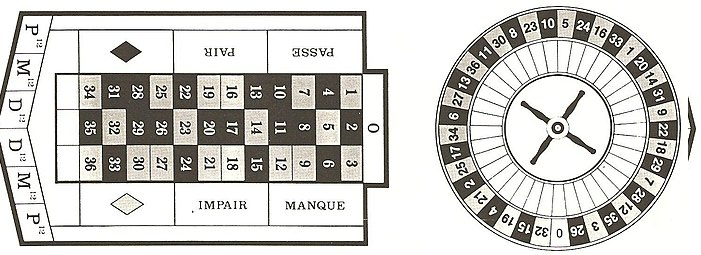
\includegraphics[width=.9\linewidth]{./figures/roulette.jpg}
\end{center}


\begin{enumerate}
\item Choosing among rewards: Roulette
\label{sec:org5efd2f7}
\begin{itemize}
\item\relax [A] Bet 10 CHF on black
\item\relax [B] Bet 10 CHF on 0
\item\relax [C] Bet nothing

\item What is the reward here?
\item What is the outcome?
\end{itemize}
\end{enumerate}
\subsubsection{Uncertain outcomes}
\label{sec:org86a592e}
\begin{itemize}
\item\relax [A] Taking the car to Zurich (50'-80' with delays)
\item\relax [B] Taking the train to Zurich (60' without delays)
\end{itemize}
What is the reward here? 

\begin{enumerate}
\item Car\hfill{}\textsc{BMCOL}
\label{sec:orge479724}
\begin{center}
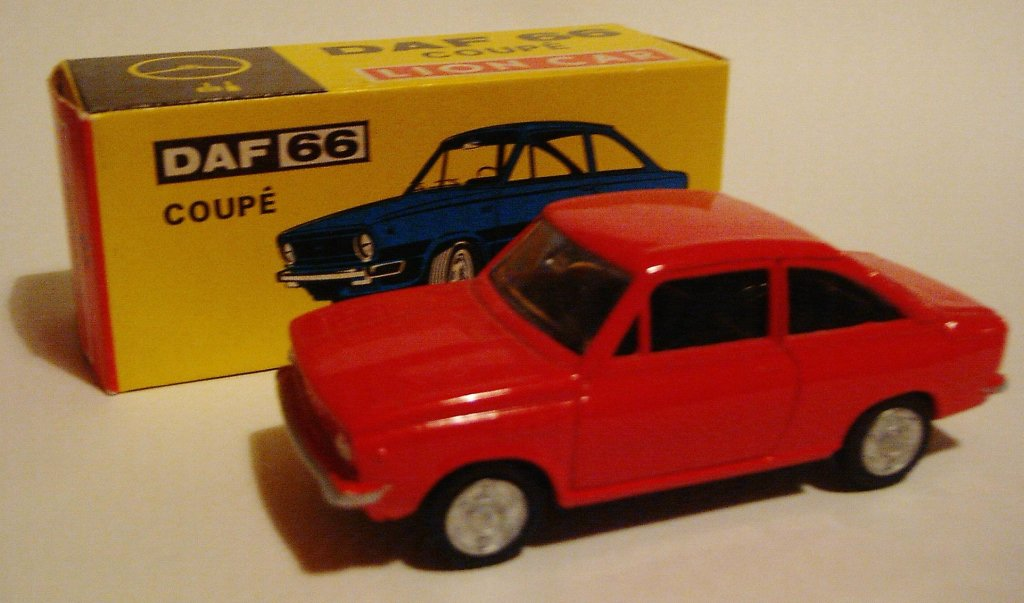
\includegraphics[width=.9\linewidth]{./figures/car.jpg}
\end{center}
\item Train\hfill{}\textsc{BMCOL}
\label{sec:org28df417}
\begin{center}
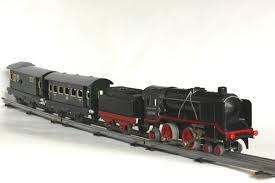
\includegraphics[width=.9\linewidth]{./figures/train.jpeg}
\end{center}
\end{enumerate}




\subsubsection{Independent outcomes}
\label{sec:org2bb79d3}

\begin{enumerate}
\item Graphical model
\label{sec:org7a233f2}
\begin{center}
      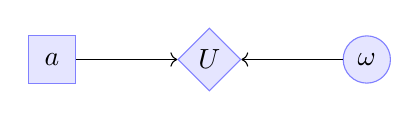
\begin{tikzpicture}
        \node[select] at (0,0) (a) {$a$};
	\node[RV] at (4,0) (w) {$\omega$};
        \node[utility] at (2,0) (U) {$U$};
	\draw[->] (a) -- (U);
	\draw[->] (w) -- (U);
      \end{tikzpicture}
\end{center}

\item Random rewards
\label{sec:org0118221}
\begin{itemize}
\item We \textbf{select} our action.
\item Outcomes are \textbf{random}, with \(\omega \sim P\), but \textbf{independent} of our action
\item We then obtain a random \textbf{utility} with distribution depending on \(a\).
\end{itemize}
\[
\Pr(U = u \mid a) = P(\{\omega : U(\omega, a) = u\})
\]
\end{enumerate}


\subsubsection{General case}
\label{sec:org57a043e}
\begin{enumerate}
\item Graphical model
\label{sec:org2add978}
\begin{center}
      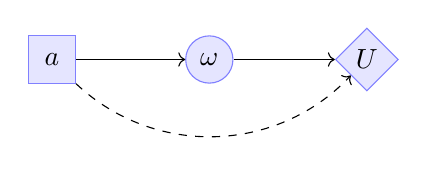
\begin{tikzpicture}
        \node[select] at (0,0) (a) {$a$};
	\node[RV] at (2,0) (w) {$\omega$};
        \node[utility] at (4,0) (U) {$U$};
	\draw[->] (a) -- (w);
	\draw[->] (w) -- (U);
	\draw[->, dashed] (a) to [bend right=45] (U);
      \end{tikzpicture}
\end{center}
\item Random rewards
\label{sec:org60dae85}
\begin{itemize}
\item We \textbf{select} our action.
\item The action determines the \textbf{outcome} distribution.
\item The utility may depend on \textbf{both} the outcome and reward.
\end{itemize}
\end{enumerate}
\subsubsection{Route selection}
\label{sec:org6a1dfc5}
\begin{enumerate}
\item Utility\hfill{}\textsc{B\_example}
\label{sec:org500bcdd}
\begin{center}
\begin{tabular}{l|rrrrrrr}
\hline
\(U(\omega, a)\) & 30' & 40' & 50' & 60' & 70' & 80' & 90'\\
\hline
Train & -1 & -2 & -5 & -10 & -15 & -20 & -30\\
Car & -10 & -20 & -30 & -40 & -50 & -60 & -70\\
\hline
\end{tabular}
\end{center}

\item Probability\hfill{}\textsc{B\_example}
\label{sec:orgc64f54f}
\begin{center}
\begin{tabular}{l|lllllll}
\hline
\(P(\omega \mid a)\) & 30' & 40' & 50' & 60' & 70' & 80' & 90'\\
\hline
Train & 0\% & 0\% & 50\% & 45\% & 4\% & 1\% & 0\%\\
Car & 0 & 40\% & 30\% & 15\% & 10\% & 3\% & 2\%\\
\hline
\end{tabular}
\end{center}

\item Expected utility
\label{sec:org748895c}

\begin{center}
\begin{tabular}{l|r}
Train & -7.8\\
Car & -20.82\\
\end{tabular}
\end{center}
\end{enumerate}

\subsubsection{Calculation in python}
\label{sec:orgcf4f602}
For discrete variables, the implemenation is easy.

\begin{enumerate}
\item Expected utility of action \(a\): \(\E_P[U |a] = \sum_{\omega \in \Omega} U(\omega, a)\).
\label{sec:org7996839}
\lstset{language=Python,label= ,caption= ,captionpos=b,numbers=none}
\begin{lstlisting}
# U: A matrix U[a, w]
# P: A matrix P[w, a]
# a: The action taken
def expected_utility(U, P, a):
	return np.dot(U[a, :],  P[:, a])
\end{lstlisting}
\item Finding the optimal action: \(a^* = \argmax_{a \in A} \E_P[U \mid a]\).
\label{sec:org9cf13bc}
\lstset{language=Python,label= ,caption= ,captionpos=b,numbers=none}
\begin{lstlisting}
# A: set of actions
def best_action(U, P, A):
	return np.argmax([expected_utility(U, P, a) for a in A])
\end{lstlisting}
\end{enumerate}

\subsection{Statistical Decision Theory}
\label{sec:orgab30b85}

\subsubsection{Expected utility}
\label{sec:orgb8acc00}
\begin{enumerate}
\item Actions, outcomes and utility
\label{sec:orgb050655}
In this setting, we obtain random outcomes that depend on our actions.
\begin{itemize}
\item Actions \(a \in A\)
\item Outcomes \(\omega \in \Omega\).
\item Probability of outcomes \(P(\omega \mid a)\)
\item Utility \(U : \Omega \alert{\times A} \to \Reals\)
\end{itemize}
\item Expected utility
\label{sec:org1c8edac}
The expected utility of an action is:
\[
\E_P[U \mid a] = \sum_{\omega \in \Omega} U(\omega \alert{, a}) P(\omega \alert{\mid a}).
\]

\item The expected utility hypothesis
\label{sec:org9ff1d85}
We prefer \(a\) to \(a'\) if and only if
\[
\E_P[U \mid a] \geq \E_P[U \mid a']
\]
\end{enumerate}

\subsubsection{Example: Betting}
\label{sec:org7280576}
In this example, probabilities reflect actual randomness

\begin{center}
\begin{tabular}{llrr}
\hline
Choice & Win Probability \(p\) & Payout \(w\) & Expected gain\\
\hline
Don't play & 0 & 0 & 0\\
Black & 18/37 & 2 & \\
Red & 18/37 & 2 & \\
0 & 1/37 & 36 & \\
1 & 1/37 & 36 & \\
\hline
\end{tabular}
\end{center}

\begin{center}
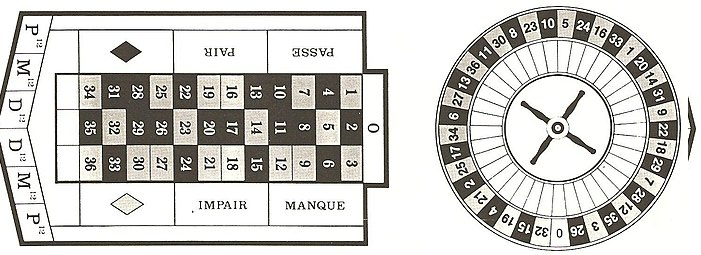
\includegraphics[width=.9\linewidth]{./figures/roulette.jpg}
\end{center}
What are the expected gains for these bets?
\subsubsection{The St-Petersburg Paradox}
\label{sec:orge323c7d}
\begin{enumerate}
\item The game
\label{sec:orgb2aae1f}
If you give me \(x\) CHF, then I promise to:
\begin{itemize}
\item (a) Throw a fair coin until it comes heads.
\item (b) If it does so after \(T\) throws, then I will give you \(2^T\) CHF.
\end{itemize}
\item The question
\label{sec:org240f844}
\begin{itemize}
\item How much \(x\) are you willing to pay to play?
\item Given that the expected amount of money is infinite, why are you only willing to pay a small \(x\)?
\end{itemize}
\end{enumerate}

\subsubsection{Example: Route selection}
\label{sec:org537c986}
\begin{itemize}
\item In this example, probabilities reflect subjective beliefs
\end{itemize}

\begin{center}
\begin{tabular}{lrlrl}
\hline
Choice & Best time & Chance of delay & Delay amount & Expected time\\
\hline
Train & 80 & 5\% & 5 & \\
Car, route A & 60 & 50\% & 30 & \\
Car, route B & 70 & 10\% & 10 & \\
\hline
\end{tabular}
\end{center}


\subsubsection{Example: Noisy optimisation}
\label{sec:org649b583}
\begin{enumerate}
\item Simple maximisation
\label{sec:orgda61b39}
For a function \(f : \Reals \to \Reals\), find a maximum \(x^*\) i.e. \(f(x^*) \geq f(x) \forall x\).
\item Necessary conditions\hfill{}\textsc{B\_theorem}
\label{sec:org28e088d}
If \(f: \Reals \to \Reals\) is a continuous function, a maximum point \(x^*\) satisfies:
\[
\frac{d}{dx} f(x^*) = 0,
\qquad
\frac{d}{dx^2} f(x^*) < 0.
\]
\item Noisy optimisation
\label{sec:orge1a7d83}
\begin{itemize}
\item We select \(x\) but \textbf{do not} observe \(f(x)\).
\item We observe a \textbf{random} \(g\) with \(\E[g | x] = f(x)\).
\end{itemize}
\begin{align}
f(x) &\defn \E[g | x],
&
\E[g | x] = \int_{- \infty}^\infty g(\omega, x) p(\omega) d\omega
\end{align}
\end{enumerate}





\subsubsection{Mean-squared error cost function}
\label{sec:org70c69ee}
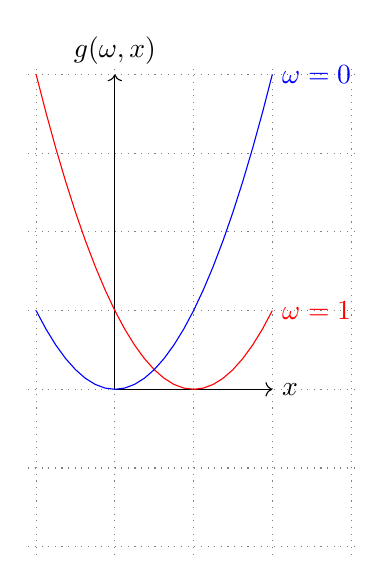
\begin{tikzpicture}[domain=-1:2, range=-1:2]
   \draw[dotted, color=gray] (-1.1,-2.1) grid (3.1,4.1);
   \draw[->] (0,0) -- (2,0) node[right] {$x$};
   \draw[->] (0,0) -- (0,4) node[above] {$g(\omega, x)$};
   \draw[color=red] plot (\x, {(\x-1)^2})  node[right] {$\omega = 1$};
   \draw[color=blue] plot (\x, {(\x)^2})  node[right] {$\omega = 0$};
\end{tikzpicture}
This example is for a quadratic loss: \(g(\omega, x) = (\omega - x)^2\).

\subsubsection{Example: Estimation}
\label{sec:org72db4bf}
\begin{itemize}
\item \(\param\): \textbf{parameter} (random)
\item \(\hat{\param}\): \textbf{estimate} (our action)
\item \((\param - \hat{\param})^2\): \textbf{cost} function
\end{itemize}
\begin{enumerate}
\item Mean-squared error minimiser
\label{sec:org72a8ddb}
If we want to guess \(\hat{\param}\), and we knew that \(\param \sim P\), then the guess
\[
\hat{\param} = \E_P(\param) = \argmin_{\hat{\param}} \E_P [(\param - \hat{\param})^2]
\]
minimises the squared error. 
This is because
\begin{align}
\frac{d}{d \hat{\theta}}
 \E_P [(\param - \hat{\param})^2]
&=
\frac{d}{d \hat{\theta}}
 \sum_\omega [\theta(\omega) -  \hat{\param}]^2 P(\omega)\\
&=
 \sum_\omega \frac{d}{d \hat{\theta}}
 [\theta(\omega) -  \hat{\param}]^2 P(\omega)\\
&=
 \sum_\omega 2 [\theta(\omega) -  \hat{\param}] (-1) P(\omega)
&=
	 2 (\hat{\param} - \E_P [\theta]).
\end{align}
Setting this to \(0\) gives \(\hat{\param} =\E_P [\theta]\)
\end{enumerate}

\section{Gradient methods}
\label{sec:org63673bc}
\subsection{Gradients for optimisation}
\label{sec:org60765cf}
\subsubsection{The gradient descent method: one dimension}
\label{sec:org922a431}
\begin{itemize}
\item Function to minimise \(f : \Reals \to \Reals\).
\item Derivative \(\frac{d}{d \param} f(\param)\)
\end{itemize}
\begin{enumerate}
\item Gradient descent algorithm
\label{sec:org185c0fb}
\begin{itemize}
\item Input: initial value \(\param^0\), \textbf{learning rate} schedule \(\alpha_t\)
\item For \(t=1, \ldots, T\)
\begin{itemize}
\item \(\param^{t+1} = \param^t - \alpha_t \frac{d}{d \param} f(\param^t)\)
\end{itemize}
\item Return \(\param^T\)
\end{itemize}
\item Properties
\label{sec:orgbf64f39}
\begin{itemize}
\item If \(\sum_t \alpha_t = \infty\) and \(\sum_t \alpha_t^2 < \infty\), it finds a local minimum \(\param^T\), i.e. there is \(\epsilon > 0\) so that
\end{itemize}
\[
f(\param^T) < f(\param), \forall \param: \|\param^T - \param\| < \epsilon.
\]
\end{enumerate}
\subsubsection{One-dimensional minimisation example}
\label{sec:orgfa5ace5}

\subsubsection{Gradient methods for expected value\hfill{}\textsc{example}}
\label{sec:org5af3f52}
\begin{enumerate}
\item Estimate the expected value
\label{sec:org5c711be}
\(x_t \sim P\) with \(\E_P[x_t] = \mu\).
\item Objective: mean squared error
\label{sec:org0e7e0e4}
Here \(\ell(x, \param) = (x - \param)^2\).
\[
\min_\param \E_P[(x_t - \param)^2].
\]
\item Exact derivative update
\label{sec:orgfa520c9}
If we know \(P\), then we can calculate
\begin{align}
\param^{t+1} &= \param^t - \alpha_t \frac{d}{d\param} \E_P[(x - \param^t)^2]\\
\frac{d}{d\param} \E_P[(x - \param^t)^2] &= 2 (\E_P[x] - \param^t)
\end{align}
\end{enumerate}

\subsubsection{Stochastic derivative}
\label{sec:orgd20c819}
\begin{itemize}
\item Function to minimise \(f : \Reals \to \Reals\).
\item Derivative \(\frac{d}{d \param} f(\param)\)
\item \(f(\param) = \E[g | \param]\)
\item \(\frac{d}{d \param} f = \E[ \frac{d}{d \param} g | \param]\)
\end{itemize}
\begin{enumerate}
\item Stochastic derivative algorithm
\label{sec:orgc54509e}
\begin{itemize}
\item Input: initial value \(\param^0\), \textbf{learning rate} schedule \(\alpha_t\)
\item For \(t=1, \ldots, T\)
\begin{itemize}
\item Observe \(g(\omega_t, \param^t\)), where \(\omega_t \sim P\).
\item \(\param^{t+1} = \param^t - \alpha_t \frac{d}{d \param} g(\omega_t, \param^t)\)
\end{itemize}
\item Return \(\param^T\)
\end{itemize}
\end{enumerate}


\subsubsection{Stochastic gradient for mean estimation}
\label{sec:org7fa3fec}
\begin{enumerate}
\item Sampling\hfill{}\textsc{B\_theorem}
\label{sec:org026069e}
For any bounded random variable \(f\), 
\[
\E_P[f] = \int_{X} dP(x) f(x)
 = 
\lim_{T \to \infty} \frac{1}{T} \sum_{t=1}^T f(x_t)
 = 
\E_P \left[\frac{1}{T} \sum_{t=1}^T f(x_t)\right]
, \qquad x_t \sim P
\]
\item Derivative ampling\hfill{}\textsc{B\_example}
\label{sec:orgf8a22f5}
We can also approximate the gradient through sampling:
\begin{align*}
 \frac{d}{d\param} \E_P [(x - \param)^2] 
&= \int_{-\infty}^\infty \!\!\!\! dP(x) \frac{d}{d\param} (x - \param)^2
\\
&\approx \frac{1}{T} \sum_{t=1}^T \frac{d}{d\param} (x_t - \param)^2
= \frac{1}{T} \sum_{t=1}^T 2(x_t - \param)
\end{align*}
\begin{itemize}
\item Wen can even update \(\param\) after \textbf{each sample} \(x_t\):
\end{itemize}
\[
\param^{t+1} = \param^t + 2 \alpha_t (x_t - \param^t)
\]
\end{enumerate}
\subsubsection{The gradient method}
\label{sec:orgb933679}
\begin{itemize}
\item Function to minimise \(f : \Reals^{\alert{n}} \to \Reals\).
\item \textbf{Gradient} \(\nabla_\param f(\param)  = \left(\frac{\partial f(\param)}{\partial \param_1}, \ldots, \frac{\partial f(\param)}{\partial \param_n}\right)\),
\item \textbf{Partial} derivative \(\frac{\partial f}{\partial \param_n}\)
\end{itemize}
\begin{enumerate}
\item Gradient descent algorithm
\label{sec:org3760df1}
\begin{itemize}
\item Input: initial value \(\param^0\), learning rate schedule \(\alpha_t\)
\item For \(t=1, \ldots, T\)
\begin{itemize}
\item \(\param^{t+1} = \param^t - \alpha_t \nabla_\param f(\param^t)\)
\end{itemize}
\item Return \(\param^T\)
\end{itemize}
\item Properties
\label{sec:org7976e1a}
\begin{itemize}
\item If \(\sum_t \alpha_t = \infty\) and \(\sum_t \alpha_t^2 < \infty\), it finds a local minimum \(\param^T\), i.e. there is \(\epsilon > 0\) so that
\end{itemize}
\[
f(\param^T) < f(\param), \forall \param: \|\param^T - \param\| < \epsilon.
\]
\end{enumerate}

\subsubsection{When the cost is an expectation\hfill{}\textsc{B\_example}}
\label{sec:org1cfa740}
In machine learning, we sometimes want to minimise the \textbf{expectation} of a \textbf{cost} \(\ell\), 
\[
f(\param) \defn \E[\ell | \param] = \int_\Omega dP(\omega) \ell(\omega, \param)
\]
This can be approximated with a sample
\[
f(\param) \approx \frac{1}{T} \sum_t \ell(\omega_t, \param)
\]
The same holds for the gradient:
\[
\nabla_\param f(\param) = \int_\Omega dP(\omega) \nabla_\param \ell(\omega, \param)
\approx \frac{1}{T} \sum_t \nabla_\param \ell(\omega_t, \param)
\]




\subsubsection{Stochastic gradient method}
\label{sec:orgcc061a4}
\begin{itemize}
\item Function to \textbf{minimise} \(f : \Reals^n \to \Reals\).
\item \textbf{Gradient} \(\nabla f(\param)\)
\item \(f(\param) = \E[\ell | \param]\)
\item \(\nabla_\param f = \E[ \nabla_\param \ell | \param]\)
\end{itemize}
\begin{enumerate}
\item Algorithm
\label{sec:orgb88a199}
\begin{itemize}
\item Input: initial value \(\param^0\), \textbf{learning rate} schedule \(\alpha_t\)
\item For \(t=1, \ldots, T\)
\begin{itemize}
\item Observe \(\ell(\omega_t, \param^t\)), where \(\omega_t \sim P\).
\item \(\param^{t+1} = \param^t - \alpha_t \nabla_\param g(\omega_t, \param^t)\)
\end{itemize}
\item Return \(\param^T\)
\end{itemize}

\item Alternative view: Noisy gradients
\label{sec:org7721a92}
\begin{itemize}
\item \(\param^{t+1} = \param^t - \alpha_t [\nabla_\param f(\param^t) + \epsilon_t]\)
\item \(\E[\epsilon_t] = 0\) is sufficient for convergence.
\end{itemize}
\end{enumerate}
\end{document}